% CSC501 Milestone 4: two report pages, then one relation/constraint page.
% Build and package: python scripts/build_m4_submission.py (repository root).
\documentclass[sigconf,nonacm]{acmart}
\settopmatter{printacmref=false,printfolios=true}
\setcopyright{none}
\renewcommand\footnotetextcopyrightpermission[1]{}
\acmDOI{}
\usepackage{xurl}
\hypersetup{hidelinks}
\urlstyle{same}
\graphicspath{{../figures/}{figures/}}
\raggedbottom
\begin{document}
\title{Dated ETF Allocation Disclosures: A Relational Design and Data-Access Layer}
\titlenote{Project repository: \url{https://github.com/Pyrex111/CSC501_Data_Modeling_Project}}
\author{Taimoor Shahzad}
\affiliation{\institution{University of Victoria}\city{Victoria}\country{Canada}}
\author{M. Shahmeer Ather Kakwan}
\affiliation{\institution{University of Victoria}\city{Victoria}\country{Canada}}
\author{Mason Li}
\affiliation{\institution{University of Victoria}\city{Victoria}\country{Canada}}
\begin{abstract}
Exchange-traded fund (ETF) allocation percentages need dates, category meanings
and source evidence to support comparison. Our relational design separates
customer holdings from provider disclosures and scopes categories by
classification edition or captured-source context. A Flask interface supports
search, creation, batch updates, deletion and dated portfolio views over a
fully synthetic dataset. Twelve tables, SQL constraints and transaction
validation preserve the modeled rules; 74 automated tests and six analytical
queries exercise the implementation. Code, setup and evaluation records:
\url{https://github.com/Pyrex111/CSC501_Data_Modeling_Project}.
\end{abstract}
\maketitle



\section{Relational Design}
% Taimoor's report contribution, 2 November 2026.
% Input into the team's ACM sigconf report; this is not a complete report.
% Add taimoor_references.bib to the team's bibliography resources.
\subsection{Relational model and integrity}
The revised ER model maps to twelve relations with thirteen foreign keys.
\texttt{Holding} represents the dated Portfolio--ETF association;
\texttt{AllocationEntry} represents a Snapshot--Category association and its
reported weight. Holding and allocation observation dates remain independent.
Each relation uses an autogenerated integer \texttt{Id}, while mandatory
business identifiers are preserved through uniqueness and non-null constraints.
These include the customer's reference number, the customer's portfolio reference,
and a company's registration number within its issuing jurisdiction.

ETF identity is supplied by its identifier records. ISIN uniqueness excludes
exchange context; ticker uniqueness includes a required exchange. Partial unique
indexes protect these alternatives and known classification editions without
inventing missing versions. A captured source is identified by URL and retrieval
time. Category identity is scoped by dimension and context: a verified scheme
edition, or an individual captured allocation block when classification is
unresolved. Identical labels across contexts do not establish equivalent meaning.

SQLite STRICT tables enforce scalar types; named checks constrain dates,
fractions and allowed values. Foreign-key enforcement is enabled per
connection~\cite{sqliteStrict,sqliteForeignKeys}. Four triggers prevent category
and snapshot dimensions from disagreeing, including after parent edits.
A validated transaction additionally checks required child records, category
contexts and complete-disclosure totals within a provisional 0.005 rounding
tolerance, pending justification from genuine source precision. These transaction rules require the supplied application boundary;
they are not database-level deferred assertions.

The schema passed 33 behavioral tests using explicitly synthetic fixtures,
including duplicate-key rejection, invalid dates/weights, dimension conflicts,
context isolation and rollback of invalid final states. These results validate
the schema contribution. Eleven additional integration regression tests passed
after correcting batch-update rollback, dated portfolio selection and missing
classification/source outputs. The quickstart now preserves existing data unless
reset is explicitly requested, and both setup paths use the validated seed loader.
The full suite now passes 74 tests: the 33 schema tests, the 11
integration regressions and 30 UI-route tests. The Flask interface is
integrated over the same parameterized operations. The retained demo source
files remain text placeholders, so file existence does not verify provider
observations.


\begin{figure*}[t]
\centering
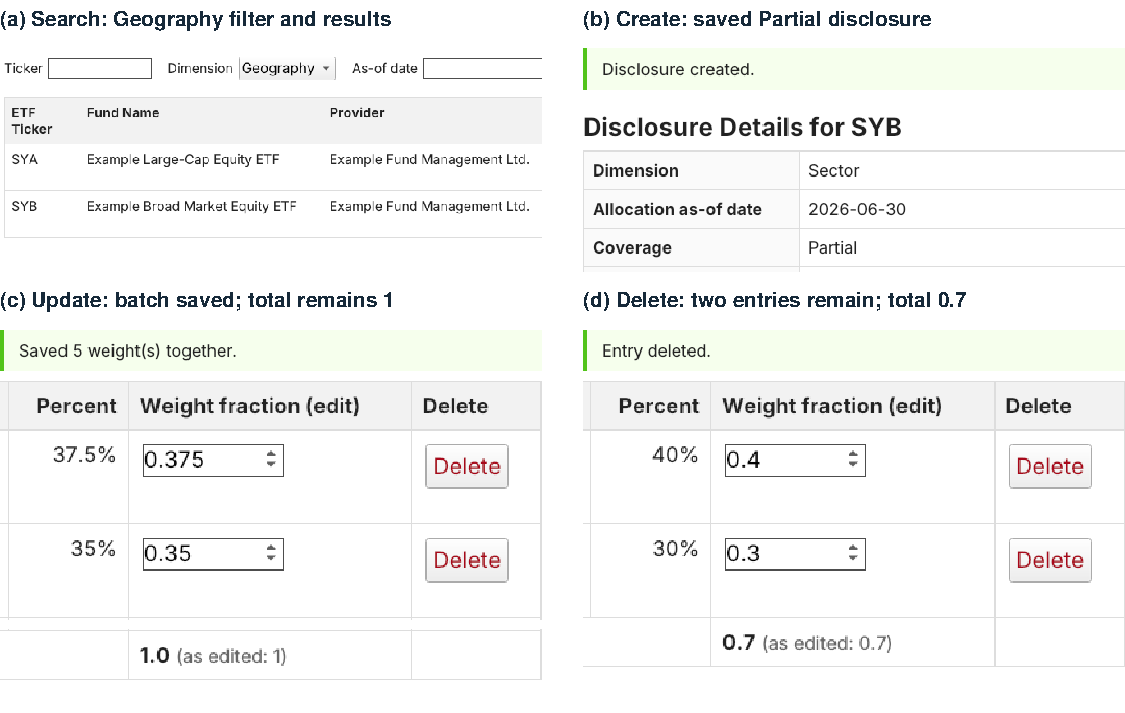
\includegraphics[width=\textwidth]{ui_operations.pdf}
\caption{Unchanged screenshot excerpts: search, successful creation, a coherent
batch update and deletion from a Partial disclosure. Intervening rows are omitted; update and delete are separate examples. All nine
full-resolution captures, including rejected writes, provenance and portfolio
views, are in \texttt{supplements/ui\_screenshots/}. All data are fictional.}
\Description{Four labeled screenshot excerpts show a Geography search, a created Partial disclosure, saved batch weights totaling one, and a deletion leaving two entries totaling 0.7.}
\label{fig:ui}
\end{figure*}
\section{Queries and Application}
% Data-access contribution: Mason; final AI-assisted condensation.
\subsection{Data and SELECT queries}
All identities and observations are fictional. Three readable synthetic PDFs
match the seed; URLs use \nolinkurl{example.invalid}. The Python loader and
\texttt{seed.sql} yield identical dumps. Every table is populated: three ETFs,
six identifiers, thirteen categories, five Complete disclosures and seventeen
entries; each Complete total is one.

Q1 joins geography entries to funds and sources (8 rows). Q2 ranks Financials
allocations within one fictional scheme edition (2). Q3 groups by snapshot
with \texttt{COUNT} and \texttt{SUM} to show coverage/totals (5). Q4 separates
observation, publication and retrieval dates (5). Q6 traces entries to category
context and retained capture (17).

Q5 returns five \emph{diagnostic candidates}: holding weight multiplied by
candidate geography allocation. For example, $0.6\times0.985=0.591$ is not
validated exposure. Look-through also requires explicit holding/disclosure
dates, coverage/basis checks and compatible category meanings. The query
retains dates and contexts instead of silently aggregating them.

\subsection{Writes and reproducibility}
INSERT, UPDATE and DELETE bind user values through parameters and use the
transaction validator. Creation saves a snapshot and entries atomically; batch edits validate the
combined result. Invalid totals or missing batch entries roll back every change.
Deletion must preserve an entry and any Complete-total requirement; successful
Partial deletion is demonstrated in Figure~\ref{fig:ui}.

After installing dependencies, \texttt{quickstart.py} builds/seeds a missing
database; \texttt{--serve} starts the UI. Later runs validate/reuse data;
only \texttt{--reset} replaces it, after a successful temporary build.
The 74 tests comprise 33 schema, 11 integration and 30 UI-route tests.
Six-query output, seed equivalence, source-PDF consistency and reuse/reset
were also verified. Synthetic checks validate behavior, not provider accuracy.

% Shahmeer: interface section (about 190 words). Figure 2 = screenshots in
% milestones/04_relational/figures/ui_screenshots/ (Mason selects panels).
\subsection{Web Interface and Validation}
The Flask interface has three layers: routes (\texttt{src/ui}), business logic (\texttt{src/biz}) and the data-access layer, so routes contain no SQL. Users search disclosures by ticker, dimension and as-of date; open a disclosure to see its basis, coverage, classification authority, scheme and version (or ``not recorded''), source URL, locator, retrieval and publication dates and retained file; create a disclosure with its entries; edit several weights together; delete an entry; and view a portfolio with the holding date shown apart from each ETF's allocation dates.

Input is checked in the browser, the business layer (real dates, fractions in $[0,1]$, no duplicate categories, at least one entry), the DAL (parameterized SQL) and the database, where \texttt{validated\_transaction} rejects any final state that breaks a rule, such as a Complete disclosure not summing to $1\pm0.005$. Rejected changes roll back and show a plain message and the user's typed values, never a server error.

We ran 30 route tests (74 with the schema suite, all passing) and exercised the running application; rejected writes left the database unchanged. Complete disclosures only accept coherent multi-entry edits, so deletion is demonstrated on a Partial synthetic disclosure.

\subsection{AI assistance and evaluation}
OpenAI ChatGPT/Codex assisted with modeling, code, tests, figures and
prose~\cite{openaiAssistance}. Taimoor's supplied critique covers keys, dates,
contexts and tolerance; Mason reports independent integrated reruns.
\href{https://github.com/Pyrex111/CSC501_Data_Modeling_Project/tree/main/milestones/04_relational}{Project evaluation records}
distinguish human review from assistant-executed checks. Personal browser
testing is not inferred.
\bibliographystyle{ACM-Reference-Format}
\bibliography{taimoor_references}
\clearpage
% Third-page fragment. In the team's ACM sigconf report, use:
% \clearpage
% % Third-page fragment. In the team's ACM sigconf report, use:
% \clearpage
% % Third-page fragment. In the team's ACM sigconf report, use:
% \clearpage
% \input{relations_constraints}
% This is the full relation/constraint listing, not a replacement for pages 1-2.
\section{Relations and constraints}
\begingroup
\emergencystretch=1em
\newcommand{\rel}[2]{\par\smallskip\noindent\textbf{#1}\par\noindent{\raggedright\ttfamily #2\par}\noindent}
\noindent
Every relation has an autogenerated \texttt{Id} INTEGER primary key.
Foreign-key columns are INTEGER; \texttt{WeightFraction} is REAL; other columns
are TEXT. Tables are STRICT. All columns are NOT NULL except those marked
\texttt{?}; required text is nonempty, and identity text has no surrounding
spaces. All FKs reference \texttt{Id}, with UPDATE/DELETE RESTRICT.
\textbf{UK} denotes uniqueness; conditional UKs apply only to their stated rows.

\rel{Customer}{Id, CustomerNumber, GivenName, FamilyName, Email?}
UK: CustomerNumber. Names and Email are not unique.

\rel{Portfolio}{Id, CustomerId, PortfolioReference, PortfolioName, BaseCurrency}
FK: CustomerId $\rightarrow$ Customer.
UK: (CustomerId, PortfolioReference).

\rel{Holding}{Id, PortfolioId, ETFId, WeightFraction, HoldingAsOfDate}
FKs: PortfolioId $\rightarrow$ Portfolio; ETFId $\rightarrow$ ETF.
UK: (PortfolioId, ETFId, HoldingAsOfDate).

\rel{ETFProvider}{Id, LegalName, RegistrationNumber, RegistrationJurisdiction, WebsiteUrl?}
UK: (RegistrationJurisdiction, RegistrationNumber).
LegalName is descriptive, not unique.

\rel{ETF}{Id, ETFProviderId, FundName, DomicileCountryCode, BaseCurrency, InceptionDate?}
FK: ETFProviderId $\rightarrow$ ETFProvider.
Business identity is supplied by ETFIdentifier; FundName is not unique.
Each saved ETF requires at least one identifier (transaction rule).

\rel{ETFIdentifier}{Id, ETFId, IdentifierScheme, IdentifierValue, ExchangeContext?}
FK: ETFId $\rightarrow$ ETF.
IdentifierScheme $\in$ \{ISIN, Ticker\}. Values are uppercase and nonempty.
ISIN: UK (IdentifierScheme, IdentifierValue), ExchangeContext is NULL;
value has 12 uppercase alphanumeric characters, two initial letters and a final
digit. Ticker: UK (IdentifierScheme, IdentifierValue, ExchangeContext);
exchange is required, uppercase and nonempty. ISIN checksum is not checked.

\par\smallskip\noindent\textbf{Common scalar rules.}
Fractions are in $[0,1]$. Currency codes have three uppercase letters and domicile
codes two. Dates are valid \texttt{YYYY-MM-DD}. Source timestamps use UTC:\\
\texttt{YYYY-MM-DDTHH:MM:SS.ffffffZ}. Optional text is NULL when unknown and
nonempty when present. Code formats do not verify external registry membership.

\newpage

\rel{SourceDocument}{Id, ETFProviderId, Url, RetrievedAt, PublishedAt?, CapturedFileRef, DocumentTitle?}
FK: ETFProviderId $\rightarrow$ ETFProvider.
UK: (Url, RetrievedAt).
CapturedFileRef identifies a retained capture; the transaction validator checks
file existence within the supplied project root.

\rel{AllocationDimension}{Id, DimensionName}
UK: DimensionName; DimensionName $\in$ \{Sector, Geography\}.

\rel{ClassificationScheme}{Id, SchemeAuthority, SchemeName, Version?, DefinitionUrl?}
Conditional UK: (SchemeAuthority, SchemeName, Version).
Applies only WHERE Version IS NOT NULL.
Unknown editions retain NULL Version and no asserted complete business key.

\rel{AllocationCategory}{Id, AllocationDimensionId, ClassificationSchemeId?, Label, Code?, ContextKey}
FKs: AllocationDimensionId $\rightarrow$ AllocationDimension;
ClassificationSchemeId $\rightarrow$ ClassificationScheme (optional).
UK: (AllocationDimensionId, ContextKey, Label).
ContextKey is generated from known authority/name/version or from captured
URL/retrieval time/block locator/dimension. Unresolved contexts are local to the
disclosure; matching labels/codes do not prove equivalence.

\rel{AllocationSnapshot}{Id, ETFId, AllocationDimensionId, SourceDocumentId, AllocationAsOfDate, BasisNote, CoverageStatus, SourceLocator}
FKs: ETFId $\rightarrow$ ETF;
AllocationDimensionId $\rightarrow$ AllocationDimension;
SourceDocumentId $\rightarrow$ SourceDocument.
UK: (ETFId, AllocationDimensionId, AllocationAsOfDate, SourceDocumentId, SourceLocator).
CoverageStatus $\in$ \{Complete, Partial, Unknown\}.
SourceLocator distinguishes dated allocation blocks/bases within a capture.

\rel{AllocationEntry}{Id, AllocationSnapshotId, AllocationCategoryId, WeightFraction}
FKs: AllocationSnapshotId $\rightarrow$ AllocationSnapshot;
AllocationCategoryId $\rightarrow$ AllocationCategory.
UK: (AllocationSnapshotId, AllocationCategoryId).

\par\smallskip\noindent\textbf{Cross-relation rules.}
SQL triggers require matching category and snapshot dimensions on entry writes and
parent dimension edits. Before COMMIT, the transaction validator requires an
entry per saved snapshot, validates used category contexts and checks Complete
totals within $0.005$ of 1 (inclusive, configurable). Partial/Unknown totals and
sampled holding totals need not equal 1. Parent minimums, contexts, totals and
file checks require the application validator; raw SQL COMMIT can bypass them.
\endgroup

% This is the full relation/constraint listing, not a replacement for pages 1-2.
\section{Relations and constraints}
\begingroup
\emergencystretch=1em
\newcommand{\rel}[2]{\par\smallskip\noindent\textbf{#1}\par\noindent{\raggedright\ttfamily #2\par}\noindent}
\noindent
Every relation has an autogenerated \texttt{Id} INTEGER primary key.
Foreign-key columns are INTEGER; \texttt{WeightFraction} is REAL; other columns
are TEXT. Tables are STRICT. All columns are NOT NULL except those marked
\texttt{?}; required text is nonempty, and identity text has no surrounding
spaces. All FKs reference \texttt{Id}, with UPDATE/DELETE RESTRICT.
\textbf{UK} denotes uniqueness; conditional UKs apply only to their stated rows.

\rel{Customer}{Id, CustomerNumber, GivenName, FamilyName, Email?}
UK: CustomerNumber. Names and Email are not unique.

\rel{Portfolio}{Id, CustomerId, PortfolioReference, PortfolioName, BaseCurrency}
FK: CustomerId $\rightarrow$ Customer.
UK: (CustomerId, PortfolioReference).

\rel{Holding}{Id, PortfolioId, ETFId, WeightFraction, HoldingAsOfDate}
FKs: PortfolioId $\rightarrow$ Portfolio; ETFId $\rightarrow$ ETF.
UK: (PortfolioId, ETFId, HoldingAsOfDate).

\rel{ETFProvider}{Id, LegalName, RegistrationNumber, RegistrationJurisdiction, WebsiteUrl?}
UK: (RegistrationJurisdiction, RegistrationNumber).
LegalName is descriptive, not unique.

\rel{ETF}{Id, ETFProviderId, FundName, DomicileCountryCode, BaseCurrency, InceptionDate?}
FK: ETFProviderId $\rightarrow$ ETFProvider.
Business identity is supplied by ETFIdentifier; FundName is not unique.
Each saved ETF requires at least one identifier (transaction rule).

\rel{ETFIdentifier}{Id, ETFId, IdentifierScheme, IdentifierValue, ExchangeContext?}
FK: ETFId $\rightarrow$ ETF.
IdentifierScheme $\in$ \{ISIN, Ticker\}. Values are uppercase and nonempty.
ISIN: UK (IdentifierScheme, IdentifierValue), ExchangeContext is NULL;
value has 12 uppercase alphanumeric characters, two initial letters and a final
digit. Ticker: UK (IdentifierScheme, IdentifierValue, ExchangeContext);
exchange is required, uppercase and nonempty. ISIN checksum is not checked.

\par\smallskip\noindent\textbf{Common scalar rules.}
Fractions are in $[0,1]$. Currency codes have three uppercase letters and domicile
codes two. Dates are valid \texttt{YYYY-MM-DD}. Source timestamps use UTC:\\
\texttt{YYYY-MM-DDTHH:MM:SS.ffffffZ}. Optional text is NULL when unknown and
nonempty when present. Code formats do not verify external registry membership.

\newpage

\rel{SourceDocument}{Id, ETFProviderId, Url, RetrievedAt, PublishedAt?, CapturedFileRef, DocumentTitle?}
FK: ETFProviderId $\rightarrow$ ETFProvider.
UK: (Url, RetrievedAt).
CapturedFileRef identifies a retained capture; the transaction validator checks
file existence within the supplied project root.

\rel{AllocationDimension}{Id, DimensionName}
UK: DimensionName; DimensionName $\in$ \{Sector, Geography\}.

\rel{ClassificationScheme}{Id, SchemeAuthority, SchemeName, Version?, DefinitionUrl?}
Conditional UK: (SchemeAuthority, SchemeName, Version).
Applies only WHERE Version IS NOT NULL.
Unknown editions retain NULL Version and no asserted complete business key.

\rel{AllocationCategory}{Id, AllocationDimensionId, ClassificationSchemeId?, Label, Code?, ContextKey}
FKs: AllocationDimensionId $\rightarrow$ AllocationDimension;
ClassificationSchemeId $\rightarrow$ ClassificationScheme (optional).
UK: (AllocationDimensionId, ContextKey, Label).
ContextKey is generated from known authority/name/version or from captured
URL/retrieval time/block locator/dimension. Unresolved contexts are local to the
disclosure; matching labels/codes do not prove equivalence.

\rel{AllocationSnapshot}{Id, ETFId, AllocationDimensionId, SourceDocumentId, AllocationAsOfDate, BasisNote, CoverageStatus, SourceLocator}
FKs: ETFId $\rightarrow$ ETF;
AllocationDimensionId $\rightarrow$ AllocationDimension;
SourceDocumentId $\rightarrow$ SourceDocument.
UK: (ETFId, AllocationDimensionId, AllocationAsOfDate, SourceDocumentId, SourceLocator).
CoverageStatus $\in$ \{Complete, Partial, Unknown\}.
SourceLocator distinguishes dated allocation blocks/bases within a capture.

\rel{AllocationEntry}{Id, AllocationSnapshotId, AllocationCategoryId, WeightFraction}
FKs: AllocationSnapshotId $\rightarrow$ AllocationSnapshot;
AllocationCategoryId $\rightarrow$ AllocationCategory.
UK: (AllocationSnapshotId, AllocationCategoryId).

\par\smallskip\noindent\textbf{Cross-relation rules.}
SQL triggers require matching category and snapshot dimensions on entry writes and
parent dimension edits. Before COMMIT, the transaction validator requires an
entry per saved snapshot, validates used category contexts and checks Complete
totals within $0.005$ of 1 (inclusive, configurable). Partial/Unknown totals and
sampled holding totals need not equal 1. Parent minimums, contexts, totals and
file checks require the application validator; raw SQL COMMIT can bypass them.
\endgroup

% This is the full relation/constraint listing, not a replacement for pages 1-2.
\section{Relations and constraints}
\begingroup
\emergencystretch=1em
\newcommand{\rel}[2]{\par\smallskip\noindent\textbf{#1}\par\noindent{\raggedright\ttfamily #2\par}\noindent}
\noindent
Every relation has an autogenerated \texttt{Id} INTEGER primary key.
Foreign-key columns are INTEGER; \texttt{WeightFraction} is REAL; other columns
are TEXT. Tables are STRICT. All columns are NOT NULL except those marked
\texttt{?}; required text is nonempty, and identity text has no surrounding
spaces. All FKs reference \texttt{Id}, with UPDATE/DELETE RESTRICT.
\textbf{UK} denotes uniqueness; conditional UKs apply only to their stated rows.

\rel{Customer}{Id, CustomerNumber, GivenName, FamilyName, Email?}
UK: CustomerNumber. Names and Email are not unique.

\rel{Portfolio}{Id, CustomerId, PortfolioReference, PortfolioName, BaseCurrency}
FK: CustomerId $\rightarrow$ Customer.
UK: (CustomerId, PortfolioReference).

\rel{Holding}{Id, PortfolioId, ETFId, WeightFraction, HoldingAsOfDate}
FKs: PortfolioId $\rightarrow$ Portfolio; ETFId $\rightarrow$ ETF.
UK: (PortfolioId, ETFId, HoldingAsOfDate).

\rel{ETFProvider}{Id, LegalName, RegistrationNumber, RegistrationJurisdiction, WebsiteUrl?}
UK: (RegistrationJurisdiction, RegistrationNumber).
LegalName is descriptive, not unique.

\rel{ETF}{Id, ETFProviderId, FundName, DomicileCountryCode, BaseCurrency, InceptionDate?}
FK: ETFProviderId $\rightarrow$ ETFProvider.
Business identity is supplied by ETFIdentifier; FundName is not unique.
Each saved ETF requires at least one identifier (transaction rule).

\rel{ETFIdentifier}{Id, ETFId, IdentifierScheme, IdentifierValue, ExchangeContext?}
FK: ETFId $\rightarrow$ ETF.
IdentifierScheme $\in$ \{ISIN, Ticker\}. Values are uppercase and nonempty.
ISIN: UK (IdentifierScheme, IdentifierValue), ExchangeContext is NULL;
value has 12 uppercase alphanumeric characters, two initial letters and a final
digit. Ticker: UK (IdentifierScheme, IdentifierValue, ExchangeContext);
exchange is required, uppercase and nonempty. ISIN checksum is not checked.

\par\smallskip\noindent\textbf{Common scalar rules.}
Fractions are in $[0,1]$. Currency codes have three uppercase letters and domicile
codes two. Dates are valid \texttt{YYYY-MM-DD}. Source timestamps use UTC:\\
\texttt{YYYY-MM-DDTHH:MM:SS.ffffffZ}. Optional text is NULL when unknown and
nonempty when present. Code formats do not verify external registry membership.

\newpage

\rel{SourceDocument}{Id, ETFProviderId, Url, RetrievedAt, PublishedAt?, CapturedFileRef, DocumentTitle?}
FK: ETFProviderId $\rightarrow$ ETFProvider.
UK: (Url, RetrievedAt).
CapturedFileRef identifies a retained capture; the transaction validator checks
file existence within the supplied project root.

\rel{AllocationDimension}{Id, DimensionName}
UK: DimensionName; DimensionName $\in$ \{Sector, Geography\}.

\rel{ClassificationScheme}{Id, SchemeAuthority, SchemeName, Version?, DefinitionUrl?}
Conditional UK: (SchemeAuthority, SchemeName, Version).
Applies only WHERE Version IS NOT NULL.
Unknown editions retain NULL Version and no asserted complete business key.

\rel{AllocationCategory}{Id, AllocationDimensionId, ClassificationSchemeId?, Label, Code?, ContextKey}
FKs: AllocationDimensionId $\rightarrow$ AllocationDimension;
ClassificationSchemeId $\rightarrow$ ClassificationScheme (optional).
UK: (AllocationDimensionId, ContextKey, Label).
ContextKey is generated from known authority/name/version or from captured
URL/retrieval time/block locator/dimension. Unresolved contexts are local to the
disclosure; matching labels/codes do not prove equivalence.

\rel{AllocationSnapshot}{Id, ETFId, AllocationDimensionId, SourceDocumentId, AllocationAsOfDate, BasisNote, CoverageStatus, SourceLocator}
FKs: ETFId $\rightarrow$ ETF;
AllocationDimensionId $\rightarrow$ AllocationDimension;
SourceDocumentId $\rightarrow$ SourceDocument.
UK: (ETFId, AllocationDimensionId, AllocationAsOfDate, SourceDocumentId, SourceLocator).
CoverageStatus $\in$ \{Complete, Partial, Unknown\}.
SourceLocator distinguishes dated allocation blocks/bases within a capture.

\rel{AllocationEntry}{Id, AllocationSnapshotId, AllocationCategoryId, WeightFraction}
FKs: AllocationSnapshotId $\rightarrow$ AllocationSnapshot;
AllocationCategoryId $\rightarrow$ AllocationCategory.
UK: (AllocationSnapshotId, AllocationCategoryId).

\par\smallskip\noindent\textbf{Cross-relation rules.}
SQL triggers require matching category and snapshot dimensions on entry writes and
parent dimension edits. Before COMMIT, the transaction validator requires an
entry per saved snapshot, validates used category contexts and checks Complete
totals within $0.005$ of 1 (inclusive, configurable). Partial/Unknown totals and
sampled holding totals need not equal 1. Parent minimums, contexts, totals and
file checks require the application validator; raw SQL COMMIT can bypass them.
\endgroup

\end{document}
